\documentclass[french,12pt,a4paper,oneside,notitlepage]{report}
\usepackage[utf8]{inputenc}
\usepackage[T1]{fontenc}
\usepackage{lmodern}
\usepackage[margin=2.5cm]{geometry}
\usepackage[french]{babel}
\usepackage{xcolor}
\usepackage{times}
\usepackage{graphicx}
\usepackage{amsthm}
\usepackage{fourier}
\usepackage{hyperref}   % links im text
\usepackage{enumerate}  % for advanced numbering of lists
\usepackage{fancyhdr}  
\usepackage{caption}
\usepackage{listings}
%\usepackage{mathtools}
\usepackage{amsmath}   %arraycolsep
\usepackage[protrusion=true,expansion=true]{microtype}
\usepackage{color}
\usepackage{pdflscape}
\makeatletter
\definecolor{bl}{rgb}{0,0.2,0.6}
\let\LaTeX@startsection\@startsection
\renewcommand{\@startsection}[6]{\LaTeX@startsection%
{#1}{#2}{#3}{#4}{#5}{\color{bl}\raggedright #6}}
\renewcommand{\thesection}{\@arabic\c@section}{\color{bl}}
\renewcommand\paragraph{\@startsection{paragraph}{4}{\z@}%
  {-3.25ex\@plus -1ex \@minus -.2ex}%
  {1.5ex \@plus .2ex}%
  {\normalfont\normalsize\bfseries}}
\makeatother

\DeclareCaptionFont{white}{\color{white}}
\DeclareCaptionFormat{listing}{%
  \parbox{\textwidth}{\colorbox{gray}{\parbox{\textwidth}{#1#2#3}}}}
\captionsetup[lstlisting]{format=listing,labelfont=white,textfont=white}
\lstset{frame=lrb,xleftmargin=\fboxsep,xrightmargin=-\fboxsep}

\lstset{
 	language=C++,
% 	captionpos=b,
 	tabsize=3,
 	frame=single,
 	xleftmargin=\fboxsep,
 	xrightmargin=-\fboxsep,
 	keywordstyle=\color{blue},
 	commentstyle=\color{gray},
 	stringstyle=\color{green},
	extendedchars=true,
% 	numbers=left,
 	numberstyle=\tiny,
 	numbersep=5pt,
 	breaklines=true,
 	showstringspaces=false,
 	basicstyle=\footnotesize\ttfamily,
 	emph={label},
 	inputencoding=utf8,
 	extendedchars=true, 	
 	  literate=%
 	  {é}{{\'{e}}}1
 	  {è}{{\`{e}}}1
 	  {ê}{{\^{e}}}1
 	  {ë}{{\¨{e}}}1
 	  {û}{{\^{u}}}1
 	  {ù}{{\`{u}}}1
 	  {â}{{\^{a}}}1
 	  {à}{{\`{a}}}1
 	  {î}{{\^{i}}}1
 	  {ç}{{\c{c}}}1
 	  {Ç}{{\c{C}}}1
 	  {É}{{\'{E}}}1
 	  {Ê}{{\^{E}}}1
 	  {À}{{\`{A}}}1
 	  {Â}{{\^{A}}}1
 	  {Î}{{\^{I}}}1	
}



%Page
% type user-defined commands here
\begin{document}
\title{RAPPORT DU PROJET \\
  Classification de documents}
\author{Rédigé par:\\
Nguyen Van Tho, Khong Minh Thanh\vspace{1cm}\\
Sous la supervision de :\\
Rémy Mullot}         
%\date{ Décembre, 2013}    % type date between braces
\date{ 1 Janvier 2014, mise à jour 10 Janvier 2014}
\maketitle

\section{Introduction}
% Demarche qui est fait
% - comment obtenir des descripteurs?
% - la methode pour reconnaitre le document
%  
% Le résultat, expérimentation, expliquer pourquoi avoir ces résultats?
% Perspective: qu'est-ce qui peut fait pour améliorer le travail?
Dans le cadre du module indexation des contenus multimédias, 
il nous a été demandé de développer un programme qui permet de classifier les documents.
Les entrées du programme, ce sont des images scannées à partir des documents réels.
En effet, il y a deux premiers types de documents que le système doit reconnaître:
 \textit{Demande de prime de déménagement} et \textit{demande d'aide }
Puis, pour les autres documents, le programme peut les classifier comme le type 3, type 4, \dots pour que nous puissions les traiter des informations.

Pour reconnaître les documents, il existe des techniques tels que OCR, SVM, naïve Bayes, extraction de caractéristiques et les comparer \dots. Dans ce travail, nous essayerons de réaliser deux méthodes : 
\begin{itemize}
\item Extraire des caractéristiques endivisant l'image en blocs
\item Extraire des caractéistiques principales par le PCA
\end{itemize}
Ensuite, nous faisons la reconnaissance des documents par le méthode 1-NN, pour les classifier, nous utilisons Kmeans

Nous utilisons les données dans le cours pour la base d'apprentissage et de test.

Afin de rendre compte du travail effectué dans ce projet, nous avons rédigé ce rapport qui
est structuré en des grandes parties :

\begin{itemize}
\item Méthodes proposées
\item Expérimentation et analyse des résultats
\end{itemize}

\pagebreak
\section{Méthodes proposées}
\subsection{Prétraitement d'images}
%\textbf{Convertir en gris, effacer le border}
En voyant que les documents donnés sont grands (la taille originale est environ 
$2480x3500$, 5 Mo), et la classification des document n'a pas besoins d’une très bonne 
qualité de l’image d’entrée, nous proposons de réduire la taille de l’image entrée (dans 
ce travail nous avons réduit 4 fois la taille des images). Nous convertissons aussi les images en couleur aux images en gris car les documents ne tienne pas compte de couleur.

De plus, en examinant des images, nous avons vu que l’entête des documents est la
partie qui représente assez informations pour la classification. Nous proposons donc de
traiter l’entête des documents. L’avantage de cette approche est que nous n’avons pas 
besoins beaucoup de calcule, et aussi le programme est invariant avec le contenus du 
document (parce que le contenu est coupé).

\subsection{Extraction de caractéristiques}
Pour faire reconnaître les documents, il a besoins d'avoir des descripteurs. Nous 
proposons d'utiliser deux méthodes: extraire des descripteurs par diviser en blocs et 
la méthode PCA (principal component analysis)
\subsubsection{Extraction de caractéristiques par diviser en blocs}
Après avoir trouvé l'entête du document, pour obtenir les caractéristiques, nous avons implémenté comme suit:
\begin{itemize}
\item Nous découpons cette entête en $m \times n$ morceaux, $m$ et $n$ ce sont des fois que nous découpons en Y axis et X axis. Dans l'implémentation nous avons utilisé $m=3$ et $n =10$, nous obtenons une caractéristiques de longueur $3\times 10$ qui présente assez les informations du document.  Ci-dessous c'est l'illustration de notre méthode:

\begin{figure}[ht]
	\begin{center}
	  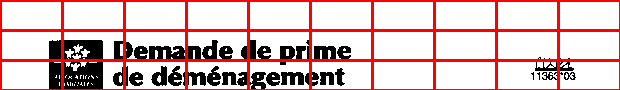
\includegraphics[width=14cm]{tete.png}
	\end{center}
	 \caption{Découpage l'entête d'un document de type 1 en $3\times 10$ morceaux
	 pour obtenir des caractéristiques}
\end{figure}


\item Pour chaque morceau nous déterminons la moyenne normalisée des pixels (on fait la
somme des pixels du morceau divisée par 255 pour la normalisation, ensuite par le nombre de pixels dans ce morceau). Ainsi pour chaque document, nous avons
$3\times 10$ valeurs permettant de le représenter (voir exemple ci-dessous)

\begin{itemize}
\item \textit{0.999461 1 1 1 1 1 1 1 1 1 1 1 0.847357 0.957389 1 0.501079 0.568501 1 0.631607 0.7411 0.964941 0.73301 0.970874 0.906149 0.462783 0.510248 0.925027 0.615426 0.75027 1  } pour l'entête ci-dessus

%\item \textit{0.986516 0.999461 1 1 1 1 1 1 1 0.908846 1 1 0.712513 1 1 0.652643 1 0.964401 0.608414 0.976268 0.880259 0.60356 0.70712 0.727077 0.624056 0.834412 0.814455 0.645092 0.998382 0.976807} pour le document de type 2
\item \dots
\end{itemize}

%double levelGray = cv::sum(image(block) / 255).val[0] / (x * y);

\end{itemize}


\subsubsection{Principal component analysis (PCA)}
PCA [1] est utilisée pour décomposer un ensemble de données à plusieurs variables en un 
ensemble de composantes orthogonales successifs qui expliquent le maximum de la variance. 
En effet, cette méthode permet d'extraire les caractéristiques d'images et à la fois 
réduire la dimension de données.

L'idée principale de cette méthode est de trouver les les composantes principales des 
images d'apprentissage. Ceci revient à déterminer les vecteurs propres de la matrice de 
covariance formée par l'ensemble des images exemples. Chaque visage exemple peut alors 
être décrit par une combinaison linéaire de ces vecteurs propres. Après avoir eu les 
vecteurs propres, on ordonne ces vecteurs par ces valeurs propres. Les vecteurs avec les 
petites valeurs propres sont supprimés. Ensuite, les images d'apprentissage et les images 
de test sont projetées sur l'espace de vecteurs propres obtenus par l'étape précédente. 
Le résultat de cette étape est les vecteurs caractéristiques des images de document.
\subsection{Classification}
L'espace de recherche dans notre problème est petite (quelques dizaines d'élément). Nous 
choisissons donc l'algorithme naïf de recherche le plus proche voisin (1-NN). Autrement 
dit, nous cherchons linéairement l'image dans la base d'apprentissage qui est plus proche 
de l'image de test (la distance euclidienne entre les deux images est plus petite). En 
fait, nous faisons deux classifications, une pour classifier l'image au type 1 ou au type 
2, si le document n'est pas un de ces deux type, la deuxième classification est utilisée 
pour classifier document à une des classes obtenues par l'étape cluster. La figure 
ci-dessous est explique le processus de classification.
\begin{figure}[ht]
	\begin{center}
	  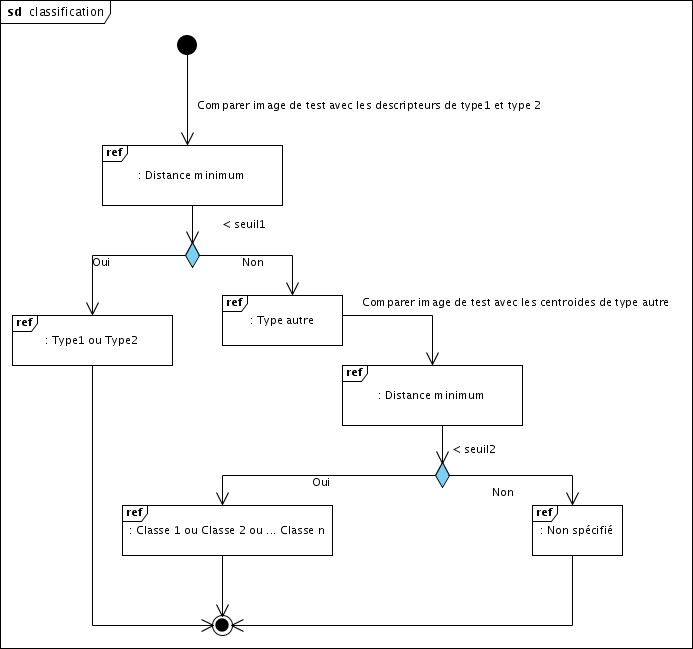
\includegraphics[width=11cm]{classification.jpg}
	\end{center}
	 \caption{Le diagramme interactif pour le processus des images}
\end{figure}

\subsection{Cluster}
Après avoir classifié les images en type 1 ou type 2, il nous reste la plupart des images 
qui n'appartiennent pas aux ces deux types. Nous devons utiliser une méthode 
d'apprentissage un-supervisé afin de regrouper ces images. Nous avons choisit la méthode 
Kmeans[2] pour cette tâche. 

\begin{figure}[ht]
	\begin{center}
	  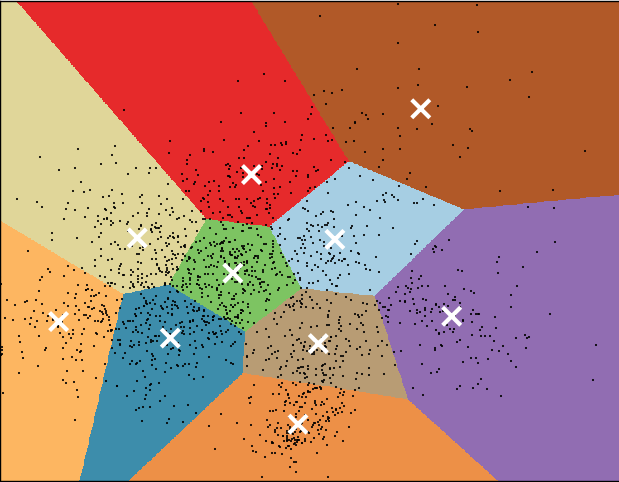
\includegraphics[width=7cm]{kmeans.png}
	\end{center}
	 \caption{La méthode Kmeans}
\end{figure}

Après avoir groupé les documents en cluster pour la base d'apprentissage, nous enregistrons les centroids de ces clusters et les réutiliserons dans la phase de test.

\section{Expérimentation}
\subsection{Indicateurs pris en compte pour l’évaluation des méthodes proposées}

Dans le but d’avoir une vue plus précise des performances de notre programme, nous
avons implémenté les indicateurs suivants :
\begin{itemize}
\item Matrice de confusion (chaque colonne de la matrice représente le nombre d’occur-
rences d’une classe estimée, tandis que chaque ligne représente le nombre d’occur-
rences d’une classe réelle (ou de référence)) : chaque élément MatriceConfusion(i,j)
de cette matrice correspond au nombre de fois où la je classe a été prédite alors que la
vraie classe était la ie. Ainsi, cet indicateur nous permet de montrer rapidement si le
système parvient à classifier correctement
\item Temps d’apprentissage du programme
\item Temps de reconnaissance Nombre de bonnes reconnaissances (good) Nombre de
mauvaises reconnaissances (bad) Taux de reconnaissance (taux) qui est le rapport
du nombre de bonnes reconnaissances par le nombre total.

\end{itemize}

\subsection{Méthode d'évaluation}
Nous appliquons la méthode d'évaluation k-fold cross validation afin d'assurer que notre 
programme va bien prédire les nouvelles données. Puisque les données proposées sont assez 
petites: 6 images pour le type 1, 6 images pour le type 2, ... nous choisissons 3 pour la 
valeur de k. Autrement, nous divisons les données en trois ensembles et chaque 
expérimentation nous prenons un ensemble  la validation et deux autres ensembles pour 
l'apprentissage. La figure ci-dessous l'explique.
\begin{figure}[ht]
	\begin{center}
	  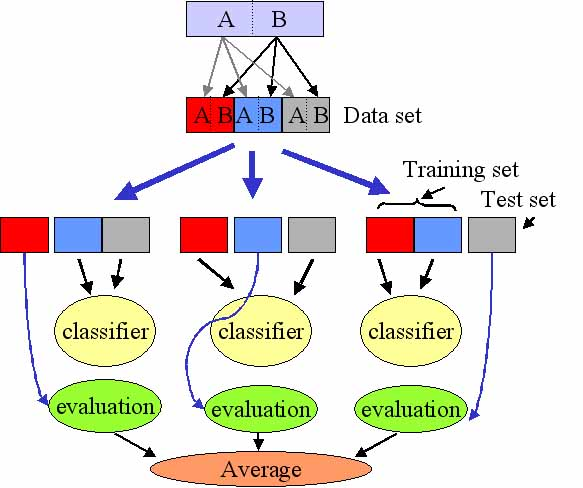
\includegraphics[width=8cm]{3fold.jpg}
	\end{center}
	 \caption{Méthode 3-fold cross validation utilisée}
	 \label{fig: 3fold validation}
\end{figure}

Pour évaluer les documents de type 1, et type 2, nous regardons seulement si leurs document sont bien classifiés dans ces types ou non. Cependant, pour les images de type autre, il faudrait avoir une autre façon d'évaluation. 

Puisque les documents de type autre ne sont pas en ordre, nous proposons d'abord de les grouper ( avec l'aide de notre programme). On voit que il y a environs 11 types de l'autre document (selon nous) tel que : \textit{UNiROSS facture, MONEY production, DELDI facture en Europe, ALLIBERT HOME France, lettre écriture, DECAYEUX,\dots}. Ensuite, dans la phase de test, si les documents sont regroupés dans une même classe, alors c'est une bonne regroupement. Au cas où il y un document qui n'est pas dans une même classe en comparaison avec notre classification, alors c'est une mauvais regroupement.
\subsection{Expérimentations}

Nous avons expérimenté deux méthode d'extraction de caractéristiques avec le Kmeans que nous avons expliqué. Un major problème de clustering avec Kmeans et de trouver le nombre de cluster optimal. Un bon choix de k est une valeur de k avec laquelle les données sont bien séparées. Nous avons observé dans les données proposées, il y a 11 classes. Nous expérimentations donc les valeurs de k de 8 à 13.
Ci-dessous notre résultat:

\subsubsection{Résultat}
\begin{table}[!ht]
  \begin{center}
	\begin{tabular}{|p{4cm}|p{2.5cm}|p{2.5cm}|p{2.7cm}|p{2.7cm}|}
	  \hline
	  Méthode & Taux de reconnaissance (type 1 + type 2) (\%) &  Taux de reconnaissance (\%) & Temps d'apprentissage (s) & Temps de reconnaissance (s)\\
	  \hline
	  blocs + K-means, k=8& 100 & 89.6 & 0.0014 & 0.00040\\
	  blocs + K-means, k=9& 100 & 85.4 & 0.0015 & 0.00042\\
	  blocs + K-means, k=10& 100 & 97.9 & 0.0016 & 0.00043\\
	  blocs + K-means, k=11& 100 & 95.8 & 0.0017 & 0.00045\\
	  blocs + K-means, k=12& 100 & 97.9 & 0.0019 & 0.00046\\
	  blocs + K-means, k=13& 100 & 97.9 & 0.0020 & 0.00048\\
	  PCA + K-means k=8& 100 & 75.0 & 0.2& 0.04\\
	  PCA + K-means k=9& 100 & 83.3 & 0.2& 0.04\\
	  PCA + K-means k=10& 100 & 89.6 & 0.2& 0.04\\
	  PCA + K-means k=11& 100 & 93.8 & 0.2& 0.04\\
	  PCA + K-means k=12& 100 & 93.8 & 0.2& 0.04\\
	  PCA + K-means k=13& 100 & 93.8 & 0.2& 0.04\\
	  \hline
	\end{tabular}
  \end{center}
  \caption{3-fold cross validation avec les valeurs de K entre 8 et 13}
\end{table}

\begin{figure}[ht]
	\begin{center}
	  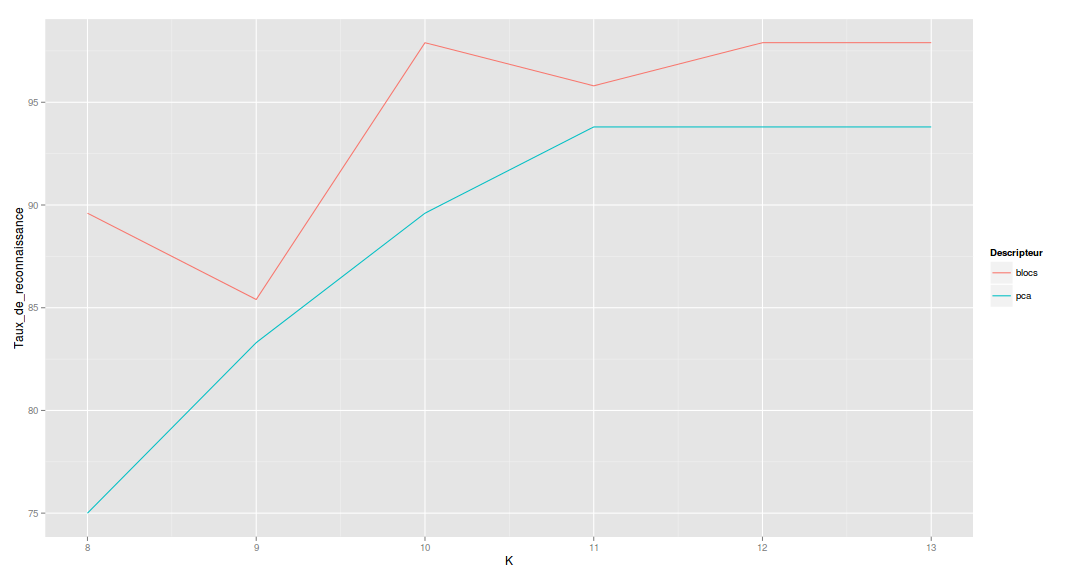
\includegraphics[width=12cm]{series.png}
	\end{center}
	 \caption{3-fold cross validation avec les valeurs de K entre 8 et 13}
	 \label{fig: K 8a13}
\end{figure}

On voit tout de suite que le résultat de reconnaissance les documents de type 1 et 2 est toujours 100\%. On constate que ces document ne varient pas beaucoup tel que la position des caractéristiques, la direction de texte, la luminance\dots De plus, nous avons déjà fait le prétraitement des documents. Les bruits sont presque éliminer, alors ces documents sont presque le même, donc le taux de 100\% est totalement réalisable. Mais s'il existe un document de ces types, qui change la position de texte, la direction de texte, nous prédisons que le taux va diminuer beaucoup.

Le taux de reconnaissance est bien dépendu à la valeur de K. En voyant le tableau ci-dessus, le résultat avec k=11 est une bonne valeur pour cluster les données, parce qu'il est le nombre de cluster de tous les ensembles de documents. La méthode de diviser en blocs ressemble mieux la méthode PCA, la raison c'est que le PCA est sensible avec les variants du document. Les documents dans une classe peut avoir la distance un peu grande, il marche donc pas très bien avec K-means. 

Un autre constat est que la méthode de diviser en blocs donne un très bon résultat, ça veut dire que le découpage en blocs de l’entête du document peut représenter plusieurs informations du document. Cela correspond bien avec la réalité où on devait écrire clairement le document dès son début.

En fin, nous voyons que le temps de calcule de méthode de diviser en blocs en plus vite que le PCA. Cela est expliqué par la projection de PCA. On doit projeter l'image entrée sur les dimensions du PCA avant de le reconnaître. Le temps de projections est en peu coûteux dans ce cas.

\begin{table}
    \begin{center}
    \resizebox{0.6\textwidth}{!}{%
        \begin{tabular}{|l|l|l|l|l|l|l|l|l|l|l|l|l|l|l|}
            \hline
            &t1 & t2 & 1 & 2 & 3 & 4 & 5 & 6 & 7 & 8 & 9 & 10 & 11 & -1\\
            \hline
            t1 & 6 & 0 & 0 & 0 & 0 & 0 & 0 & 0 & 0 & 0 & 0 & 0 & 0 & 0\\
            \hline
            t2 & 0 & 6 & 0 & 0 & 0 & 0 & 0 & 0 & 0 & 0 & 0 & 0 & 0 & 0\\
            \hline
            1 & 0 & 0 & 8 & 0 & 0 & 0 & 0 & 0 & 0 & 0 & 0 & 0 & 0 & 0\\
            \hline
            2 & 0 & 0 & 0 & 5 & 0 & 0 & 0 & 0 & 0 & 0 & 0 & 0 & 0 & 1\\
            \hline
            3 & 0 & 0 & 0 & 0 & 6 & 0 & 0 & 0 & 0 & 0 & 0 & 0 & 0 & 0\\
            \hline
            4 & 0 & 0 & 0 & 0 & 0 & 6 & 0 & 0 & 0 & 0 & 0 & 0 & 0 & 0\\
            \hline
            5 & 0 & 0 & 0 & 0 & 0 & 0 & 5 & 0 & 0 & 0 & 0 & 0 & 0 & 0\\
            \hline
            6 & 0 & 0 & 0 & 0 & 0 & 0 & 0 & 5 & 0 & 0 & 0 & 0 & 0 & 0\\
            \hline
            7 & 0 & 0 & 0 & 0 & 0 & 0 & 0 & 0 & 5 & 0 & 0 & 0 & 0 & 0\\
            \hline
            8 & 0 & 0 & 0 & 0 & 0 & 0 & 0 & 0 & 0 & 4 & 0 & 0 & 0 & 0\\
            \hline
            9 & 0 & 0 & 0 & 0 & 0 & 0 & 0 & 0 & 0 & 0 & 2 & 0 & 0 & 0\\
            \hline
            10 & 0 & 0 & 0 & 0 & 0 & 0 & 0 & 0 & 0 & 0 & 0 & 0 & 1 & 0\\
            \hline
            11 & 0 & 0 & 0 & 0 & 0 & 0 & 0 & 0 & 0 & 0 & 0 & 0 & 1 & 0\\
            \hline
        \end{tabular}
        }
    \end{center}
	\caption{Matrice de confusion avec la méthode divisé en blocs + K-means, k = 11}
\end{table}

\begin{table}[!ht]
    \begin{center}
    \resizebox{0.6\textwidth}{!}{%
        \begin{tabular}{|l|l|l|l|l|l|l|l|l|l|l|l|l|l|l|}
            \hline
            &t1 & t2 & 1 & 2 & 3 & 4 & 5 & 6 & 7 & 8 & 9 & 10 & 11 & -1\\
            \hline
            t1 & 6 & 0 & 0 & 0 & 0 & 0 & 0 & 0 & 0 & 0 & 0 & 0 & 0 & 0\\
            \hline
            t2 & 0 & 6 & 0 & 0 & 0 & 0 & 0 & 0 & 0 & 0 & 0 & 0 & 0 & 0\\
            \hline
            1 & 0 & 0 & 8 & 0 & 0 & 0 & 0 & 0 & 0 & 0 & 0 & 0 & 0 & 0\\
            \hline
            2 & 0 & 0 & 0 & 6 & 0 & 0 & 0 & 0 & 0 & 0 & 0 & 0 & 0 & 0\\
            \hline
            3 & 0 & 0 & 0 & 0 & 6 & 0 & 0 & 0 & 0 & 0 & 0 & 0 & 0 & 0\\
            \hline
            4 & 0 & 0 & 0 & 0 & 0 & 6 & 0 & 0 & 0 & 0 & 0 & 0 & 0 & 0\\
            \hline
            5 & 0 & 0 & 0 & 0 & 0 & 0 & 5 & 0 & 0 & 0 & 0 & 0 & 0 & 0\\
            \hline
            6 & 0 & 0 & 0 & 0 & 0 & 0 & 0 & 5 & 0 & 0 & 0 & 0 & 0 & 0\\
            \hline
            7 & 0 & 0 & 0 & 0 & 0 & 0 & 0 & 0 & 4 & 0 & 0 & 0 & 0 & 0\\
            \hline
            8 & 0 & 0 & 0 & 0 & 0 & 0 & 0 & 0 & 0 & 4 & 0 & 0 & 0 & 0\\
            \hline
            9 & 0 & 0 & 0 & 0 & 2 & 0 & 0 & 0 & 0 & 0 & 0 & 0 & 0 & 0\\
            \hline
            10 & 0 & 0 & 0 & 0 & 0 & 0 & 0 & 0 & 0 & 0 & 0 & 1 & 0 & 0\\
            \hline
            11 & 0 & 0 & 0 & 0 & 1 & 0 & 0 & 0 & 0 & 0 & 0 & 0 & 0 & 0\\
            \hline
        \end{tabular}
        }
    \end{center}
    \caption{Matrice de confusion PCA, Kmeans avec k = 11}
\end{table}
\clearpage
\subsubsection{ Analyses}
Au vu des matrices de confusion, nous constatons qu'il y a la confusion entre classe 10 et classe 11. Cela pourrait se justifier par le fait que la classe 10 et classe 11 n'a qu'une seul instance, la confusion est donc inévitable pour ces deux classe. 
De plus, la qualité des images, la différence de luminance, des bruits peuvent avoir des influence sur la précision de la classification et le regroupement. 

\section{Conclusion et Perspective}
Dans ce projet nous avons implémenté un programme qui permet de classifier les images de document. Afin de classifier  les documents qui ne sont pas étiquetés, notre programme a un module d'apprentissage un-supervisé basant sur la méthode Kmeans qui regroupe ces documents. 

Nous avons aussi utilisé deux méthodes différentes pour décrire les caractéristiques d'images et pour réduire la dimension de données: division d'image en blocs, PCA.
À partir des résultats de notre expérimentation, nous constatons que les documents de classe 1 et 2, les algorithmes proposées marche très bien avec un taux de reconnaissance 100\%. Par contre, pour la deuxième partie, le regroupement des images, le descripteur basant sur la division d'image en blocs est supérieur à la descripteur PCA. 
La méthode de découpage en blocs ne marche pas bien quand on donne les documents qui sont coupés la borne, ou si les documents à reconnaître change la direction.

Nous constatons que la taille de données est petite, pour améliorer la précision du programme, on peut générer des images à partir des images originales en changeant la luminance, le contraste ou le floue gaussien. Faute du temps, nous laissons cela comme un travail dans le futur.
\pagebreak
\section*{Références}
[1] Wold, Svante, Kim Esbensen, and Paul Geladi. "Principal component analysis." 
Chemometrics and intelligent laboratory systems 2.1 (1987): 37-52.

[2]Hartigan, John A., and Manchek A. Wong. "Algorithm AS 136: A k-means clustering algorithm." Journal of the Royal Statistical Society. Series C (Applied Statistics) 28.1 (1979): 100-108.
\end{document}
